\begin{figure}
  \centering 
  \begin{subfigure}[b] 
{0.45\textwidth}
    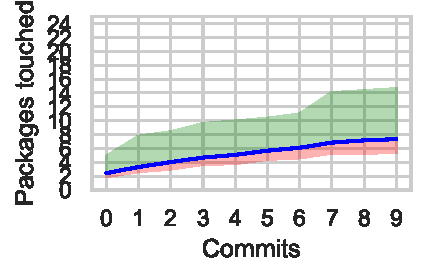
\includegraphics{sections/results/packages/time_series_components_touched.packages.all.founders.commits_10.pdf}
    \caption{Packages for All founders (n=75, $\mu$=7.39, median=4.0 \& std=5.2)}
    \label{figure.sections/results/packages/time_series_components_touched.packages.all.founders.commits_10.pdf}
  \end{subfigure}
  \begin{subfigure}[b] 
{0.45\textwidth}
    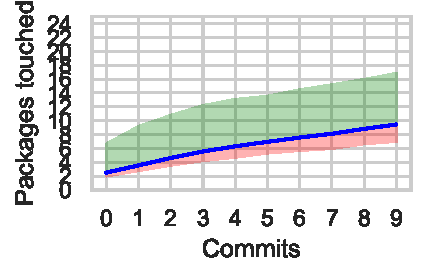
\includegraphics{sections/results/packages/time_series_components_touched.packages.all.joiners.commits_10.pdf}
    \caption{Packages for All joiners (n=849, $\mu$=9.4, median=5.0 \& std=6.27)}
    \label{figure.sections/results/packages/time_series_components_touched.packages.all.joiners.commits_10.pdf}
  \end{subfigure}
\newpage 
\vspace{3mm}
  \begin{subfigure}[b] 
{0.45\textwidth}
    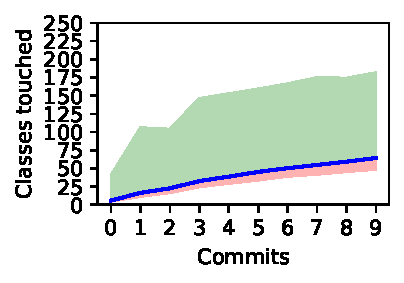
\includegraphics{sections/results/classes/time_series_components_touched.classes.all.founders.commits_10.pdf}
    \caption{Classes for All founders (n=75, $\mu$=64.4, median=17.0 \& std=70.95)}
    \label{figure.sections/results/classes/time_series_components_touched.classes.all.founders.commits_10.pdf}
  \end{subfigure}
  \begin{subfigure}[b] 
{0.45\textwidth}
    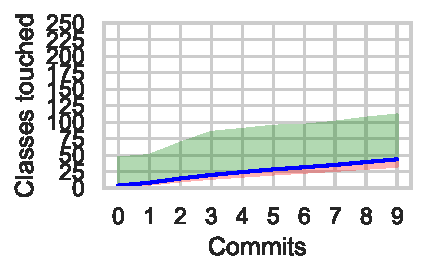
\includegraphics{sections/results/classes/time_series_components_touched.classes.all.joiners.commits_10.pdf}
    \caption{Classes for All joiners (n=849, $\mu$=43.67, median=14.0 \& std=40.97)}
    \label{figure.sections/results/classes/time_series_components_touched.classes.all.joiners.commits_10.pdf}
  \end{subfigure}
\newpage 
\vspace{3mm}
  \begin{subfigure}[b] 
{0.45\textwidth}
    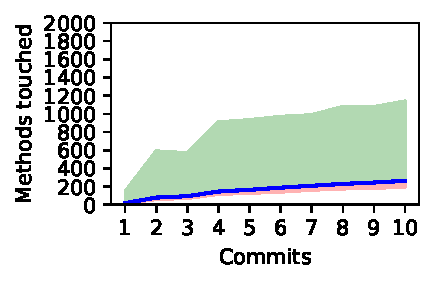
\includegraphics{sections/results/methods/time_series_components_touched.methods.all.founders.commits_10.pdf}
    \caption{Methods for All founders (n=75, $\mu$=261.01, median=46.0 \& std=414.75)}
    \label{figure.sections/results/methods/time_series_components_touched.methods.all.founders.commits_10.pdf}
  \end{subfigure}
  \begin{subfigure}[b] 
{0.45\textwidth}
    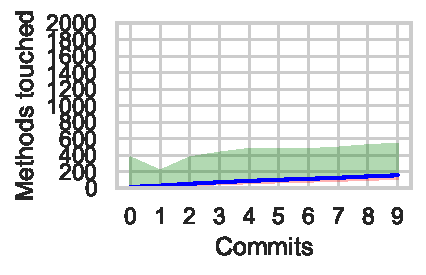
\includegraphics{sections/results/methods/time_series_components_touched.methods.all.joiners.commits_10.pdf}
    \caption{Methods for All joiners (n=849, $\mu$=155.65, median=37.0 \& std=199.82)}
    \label{figure.sections/results/methods/time_series_components_touched.methods.all.joiners.commits_10.pdf}
  \end{subfigure}
\caption{A time series for the ten (10) commits, excluding transient, with the average mean (blue line), all components touched (y-axis) against the number of commits (x-axis) for four (4) developer categories. Green is the standard deviation above the mean, and pink is the standard deviation below the mean.}\end{figure}
\clearpage 
\newpage 
